\section{Angular dependency of the Rutherford cross section}
Rutherford scattering cross section \parencite[p. 16]{noteBB} is given by
\begin{align}
    {\left( \diff[d]{\sigma}{\Omega} \right)}_|Rutherford| =
    {\left(\frac{Z_1Z_2 e^2}{4E_{\infty}} \right)}^2
    \frac{1}{{{\sin}^4(\frac{\theta}{2})}}
\end{align}
where $Z$ is the proton number of each interacting particle, $E_{\infty}$ is
the asymptotic energy, and $\theta$ is the scattering angle. If the energy is
in $\si{\mega\electronvolt}$, this differential cross section will be in
$\si{\milli\barn\per\steradian}$.

\fxnote{Jeg var træt. dette skal rettees til}
This formula neglect the recoil energy given to the target.



\subsection{Meassurements}
To test the angular dependency of the Rutherford cross section, we set the
Silicium detector at different angles.

The incomming beam will collide with both layers of the target. As the
Rutherford scattering is a coulomb interaction, we expect the gold layer to
scatter the most at higher angles.

To change the direction of the incomming proton ion, a big potential has to be
generated by the target, much similar to the motion os comets closing in on the
sun to leave it again. If not big enough the projectile will not change
direction. As it is a coulomb interaction, the 

However small, as the target has two layers, we will expect a double scattering. However







We meassured count numbers of the collector. The collector counted $10^{11}$
counts per coulomb, and as there are $6,24150913\ \cdot10^{18}$ elementary
charges per coulomb, we can related the count number to an amount of detected
protons.

Now looking at data, one sees it is not a simple gaussian distribution. This is
a consequense of a double layered target, such the incomming hydrogen ion will
scatter of both Carbon and Gold. Fitting a double gaussian, one gather
six parameters. Amplitude, centroid and standard deviation of both gaussians.
Here we use the linear combination of the two scattering processes. 

Notice that the gaussian of greatest amplitude is corresponding to gold, which
is in agreement with the relative sizes of the two atoms. Stable isotopes of
gold has a nuclear number of $A_|Au| = 197$ whereas carbon has $A_|C| = 12$.

What is interestinglt is how the two peaks change relative position as a
function of scattering, merging their gaussian distribution at low angles, and
seperating at higher angles. 

\begin{figure*}
\centering
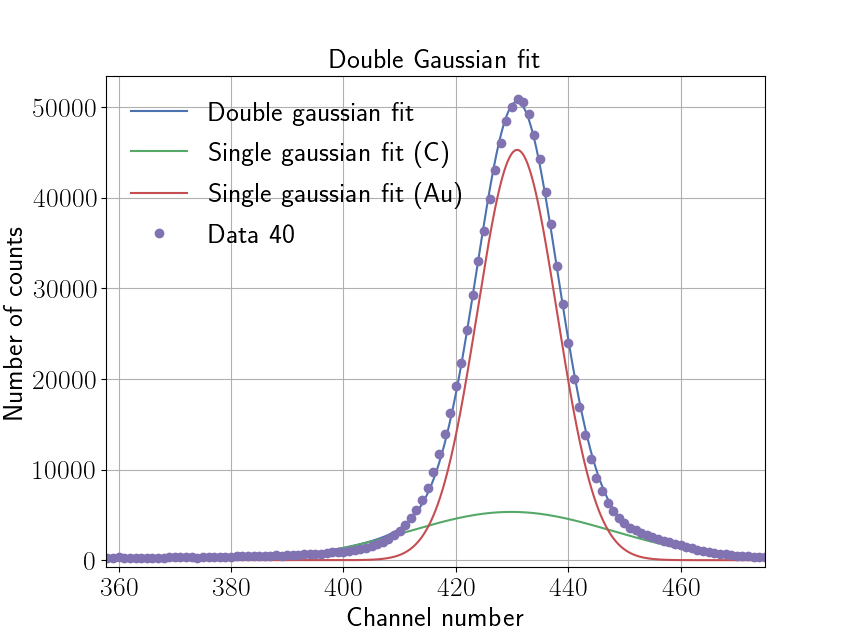
\includegraphics[width=0.99\columnwidth]{Data_40}
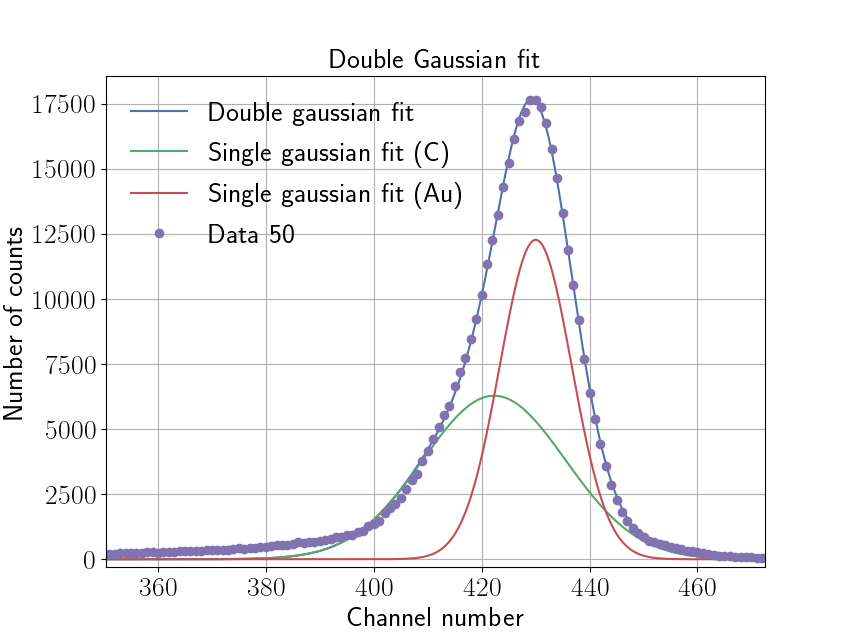
\includegraphics[width=0.99\columnwidth]{Data_50}
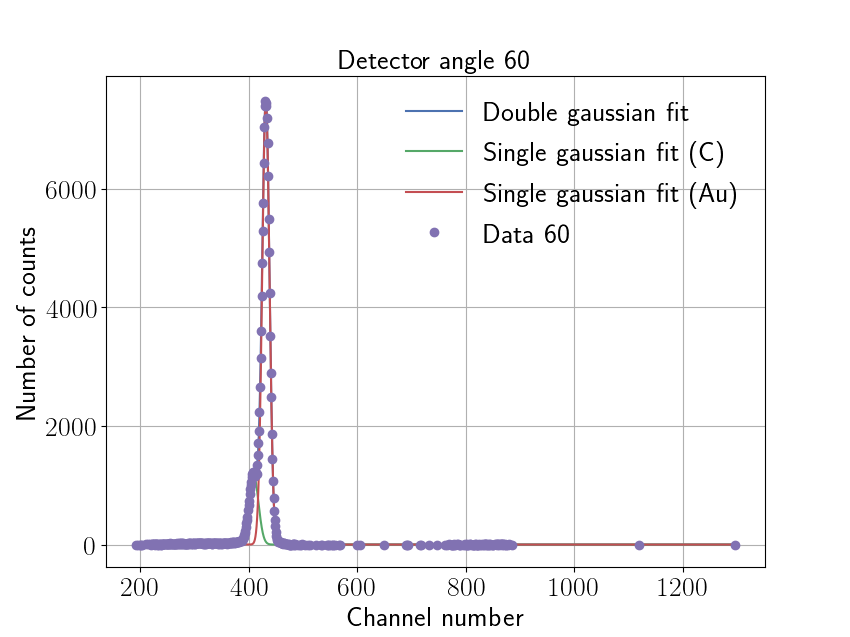
\includegraphics[width=0.99\columnwidth]{Data_60}
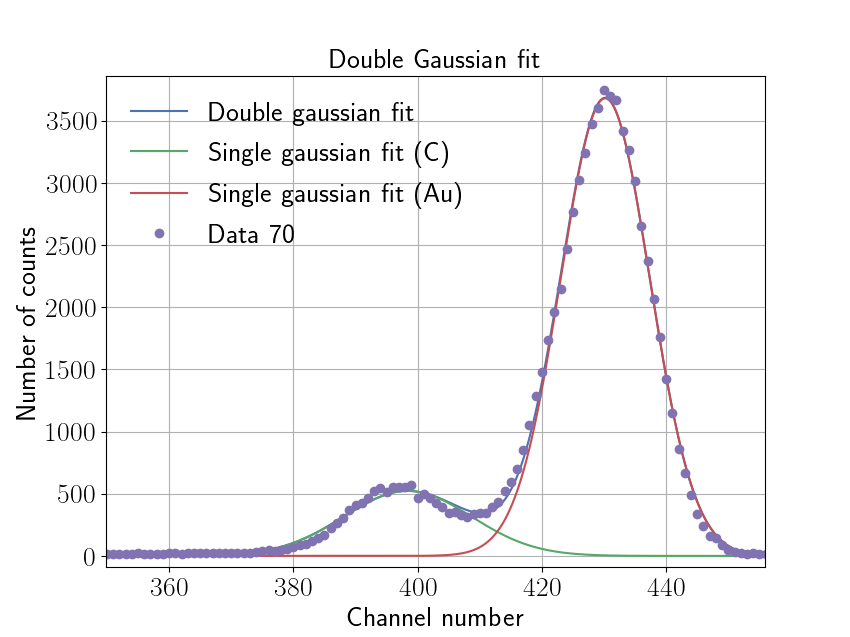
\includegraphics[width=0.99\columnwidth]{Data_70}
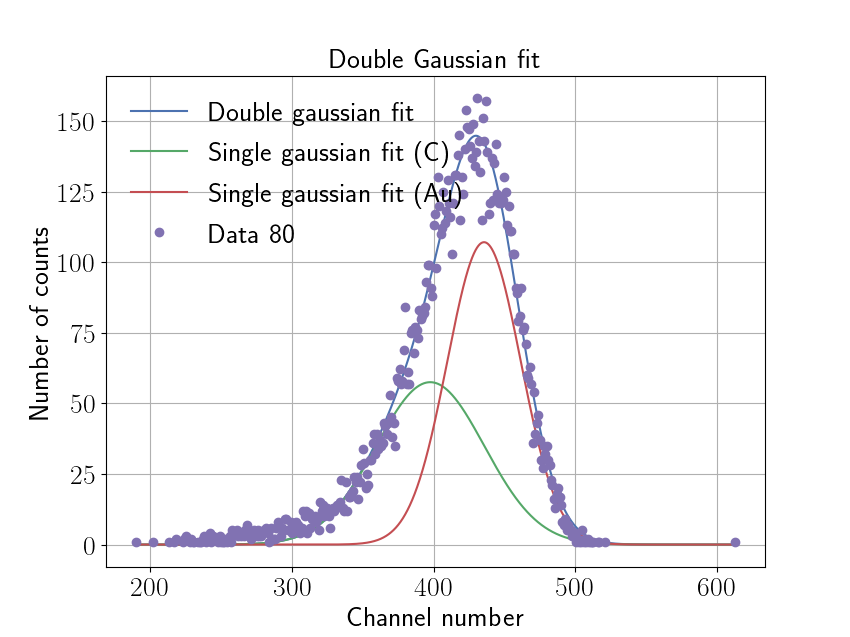
\includegraphics[width=0.99\columnwidth]{Data_80}
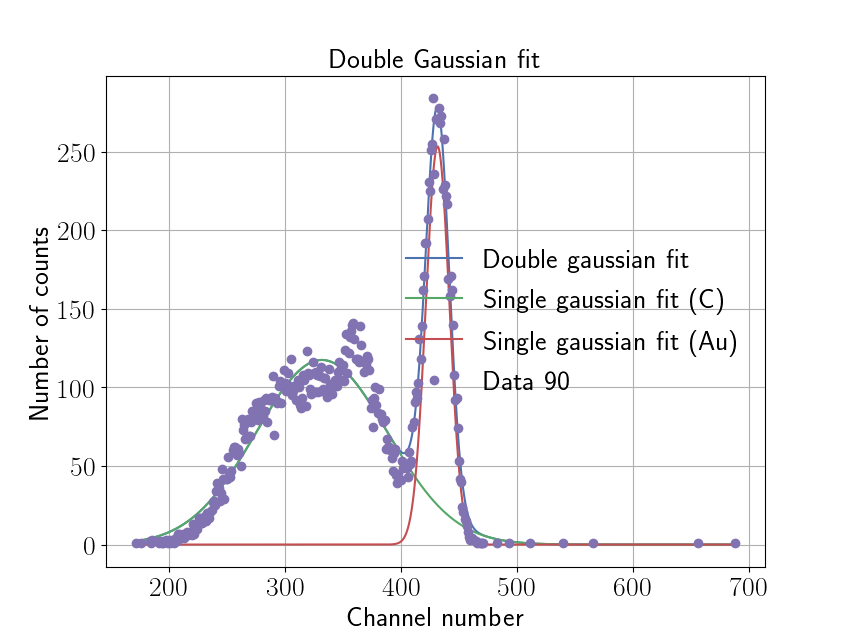
\includegraphics[width=0.99\columnwidth]{Data_90}
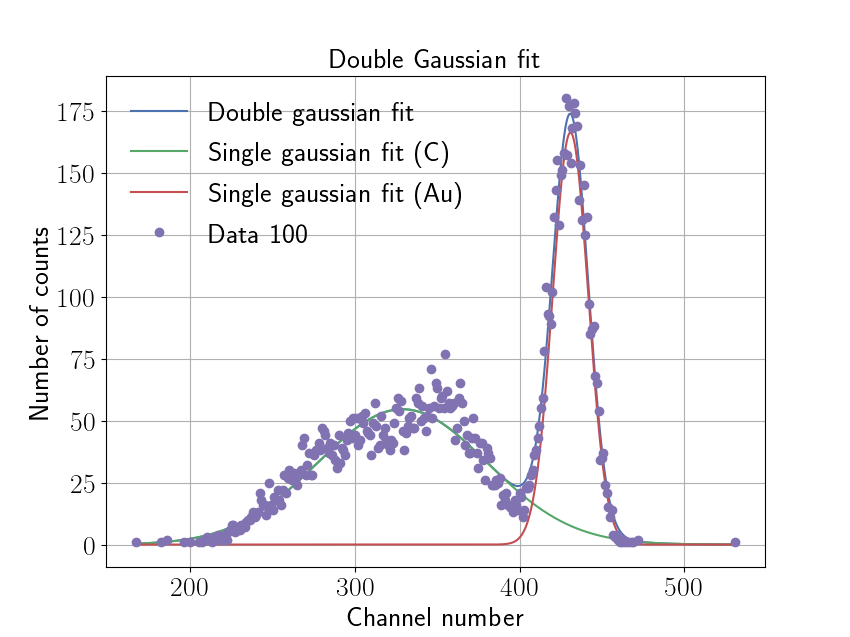
\includegraphics[width=0.99\columnwidth]{Data_100}
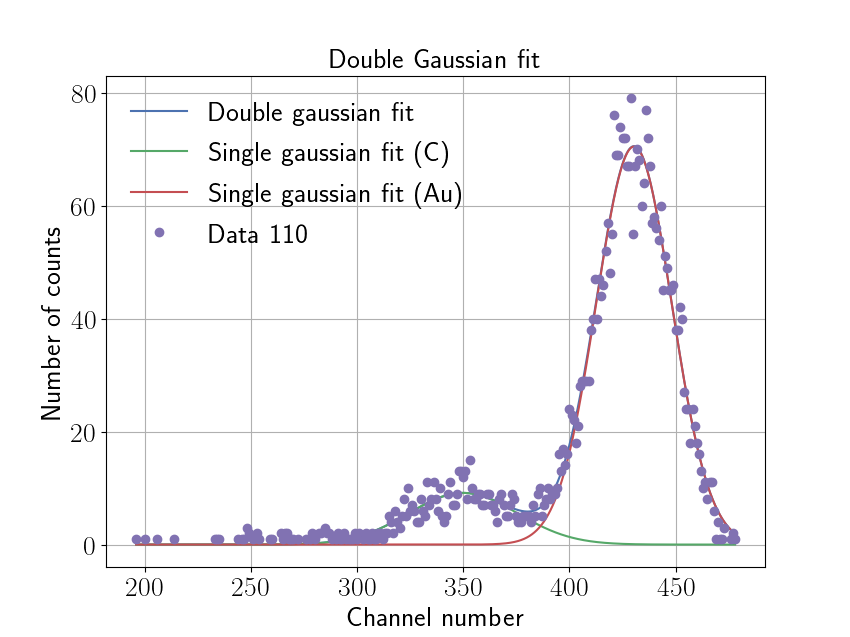
\includegraphics[width=0.99\columnwidth]{Data_110}
\label{fig_angular_dependency}
\end{figure*}

\begin{figure*}
    \centering
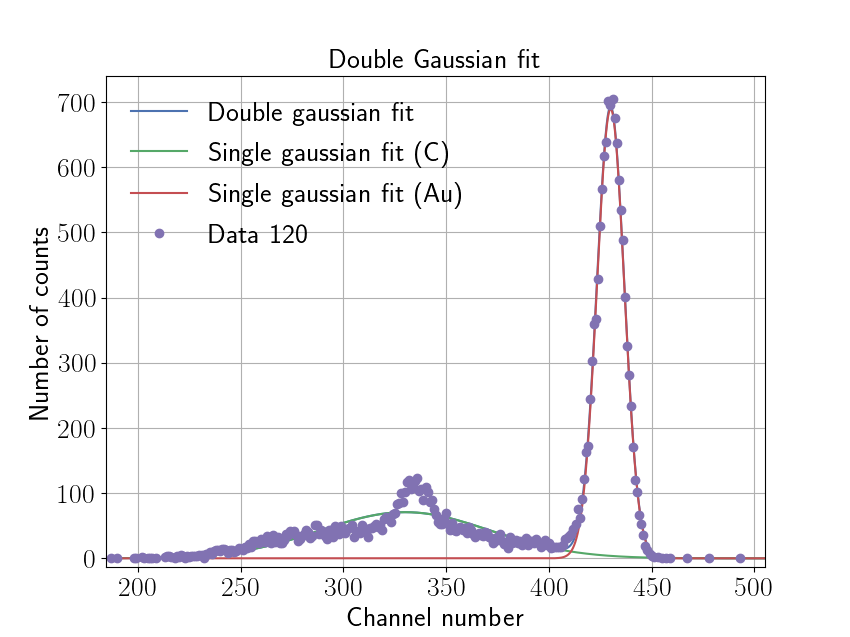
\includegraphics[width=0.99\columnwidth]{Data_120}
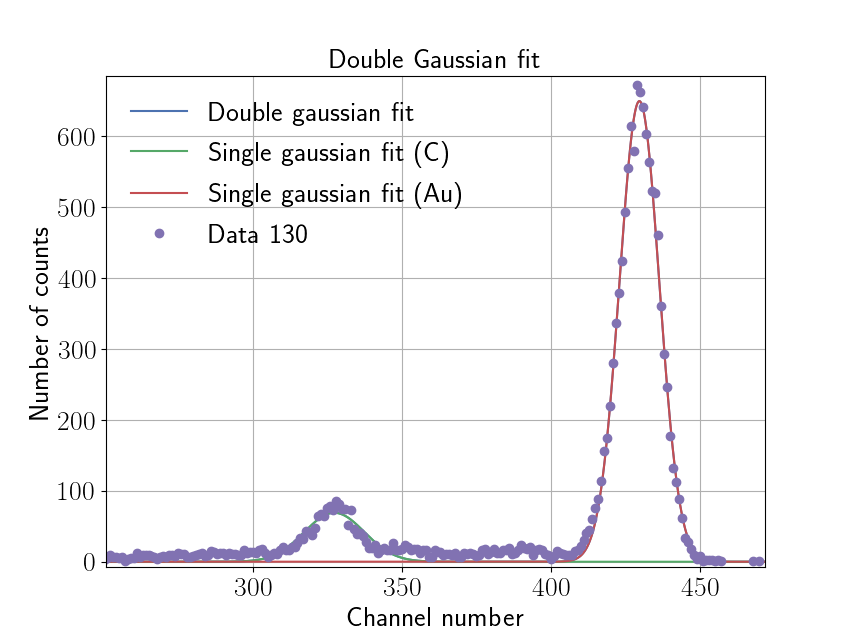
\includegraphics[width=0.99\columnwidth]{Data_130}
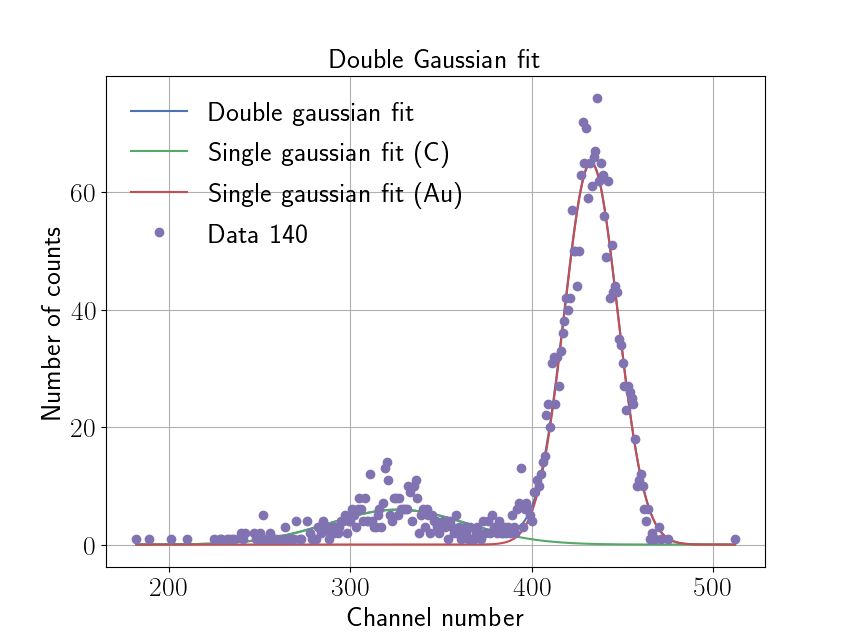
\includegraphics[width=0.99\columnwidth]{Data_140}
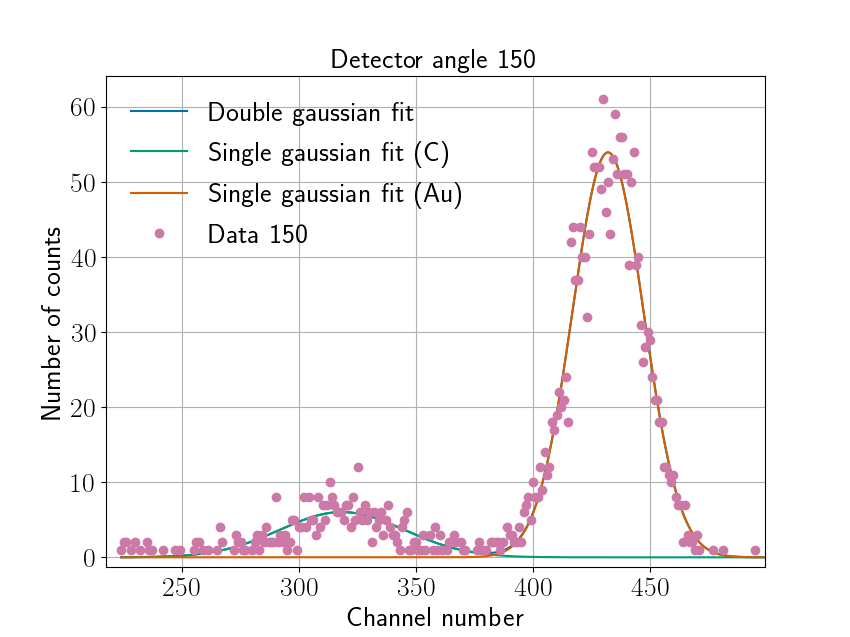
\includegraphics[width=0.99\columnwidth]{Data_150}
\label{fig_angular_dependency2}
\caption{Angular dependency}
\end{figure*}


\begin{figure}[h]
	\centering
		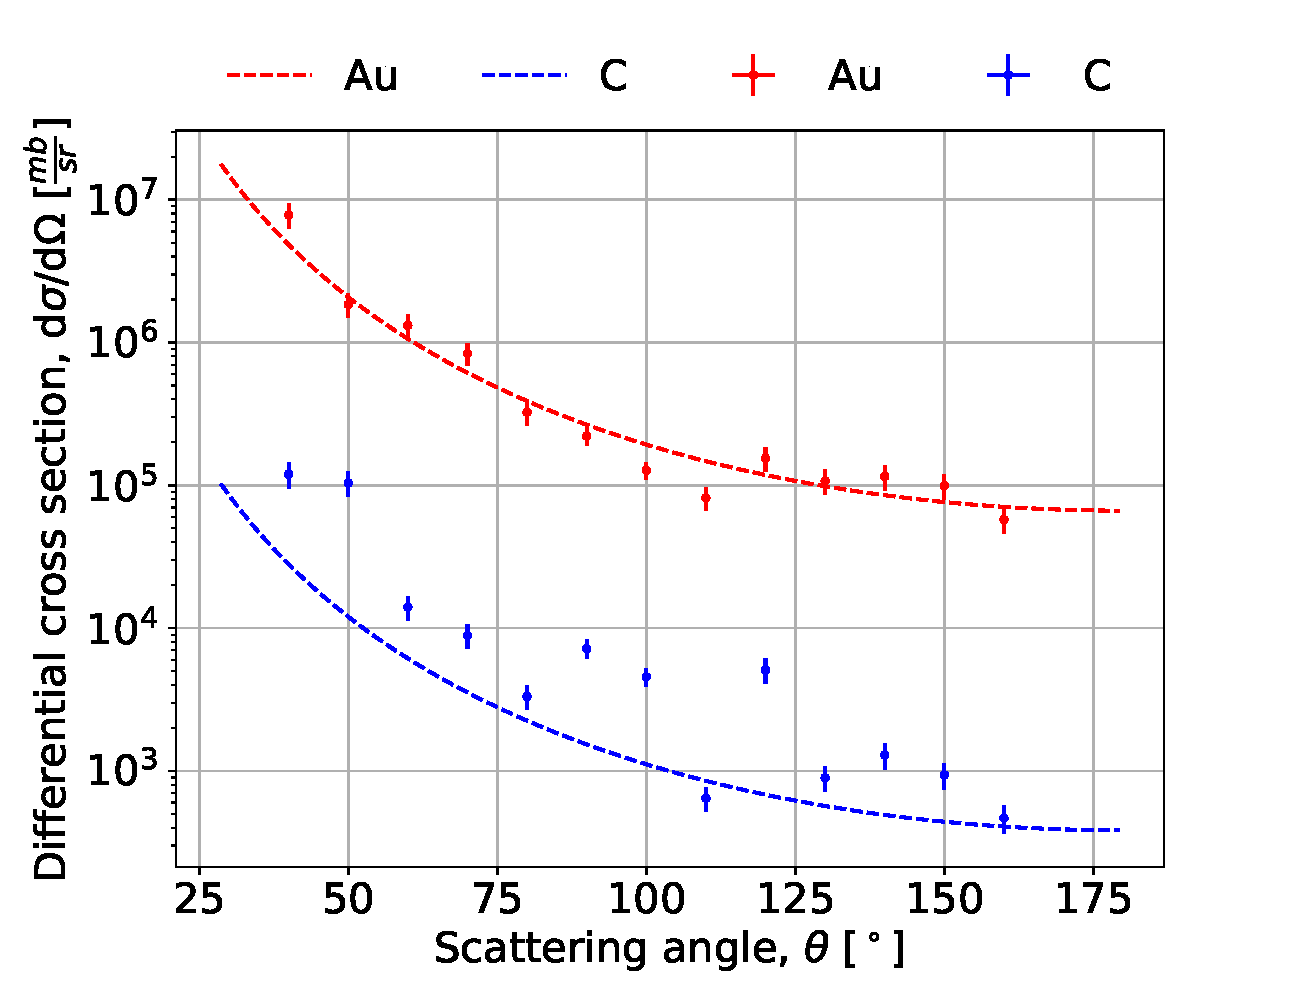
\includegraphics[width=0.45\textwidth]{Differential_cross_section.eps}
	\caption{bb}
	\label{fig:Differential_cross_section}
\end{figure}

Using the calibration to convert the centroid channel number of each gaussian,
we can plot the energies as a function of scattering angle.

\begin{figure}[h!]
\centering
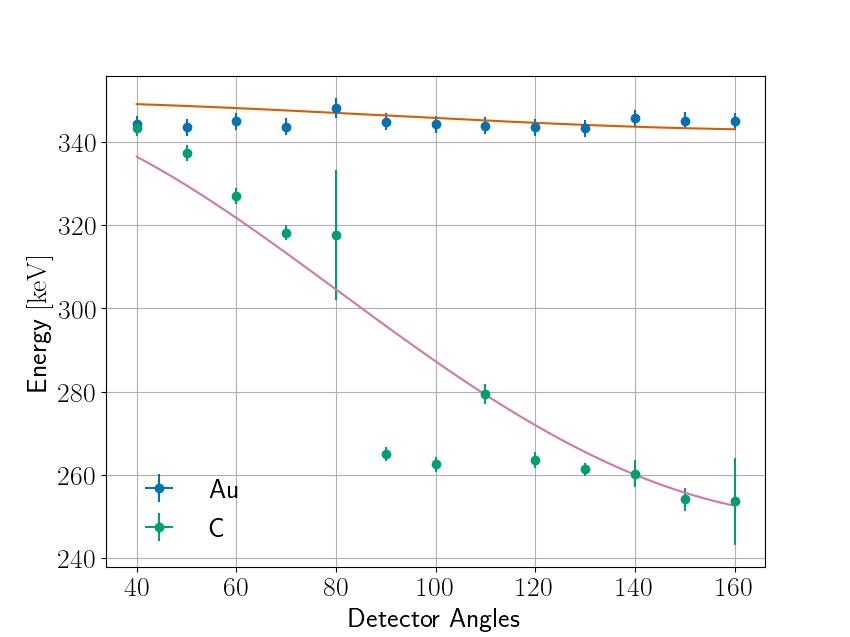
\includegraphics[width=0.99\columnwidth]{fig_energy}
\caption{Energies of Carbon and Gold scattered compared to theoretical
function.}
\label{fig_energy}
\end{figure}


The detector was at a constant seperation from the target, $r =
\SI{49\pm1}{\milli\meter}0$, and it had a circular
area of given diameter $Ø=2r=D=\SI{1.88 \pm 0.01}{\milli\meter}$ which then
gives a solid angle of
\begin{equation}
d\Omega = \frac{dA}{r^2}
\end{equation}

by using the density $\rho$ of the target $\si{\kg\per\cubic\meter}$ 


\newpage
